\section{Further analysis}
\label{sec:sensitivity}

In this section we perform an empirical analysis of the effects caused by varying the robustness hyperparameter. As can be observed in~\cref{fig:beta_sens}, in the case of Gaussian mean inference under structured contamination, setting $\beta$ to large values ($\beta \geq 0.3$) implies a more conservative summarization scheme and more rigid coreset posteriors, that do not allow good approximation quality, however maintain similar performance and small variance for increasing size of the contaminated component. For smaller $\beta$s, the KL divergence between the approximate and the true posterior can reach lower minima, however eventually the coreset quality might present larger variance, as the summarization becomes prone to adding outliers. At the remainder of the experiments, where inference is done in the presence of unstructured outliers, the effects of varying the robustness hyperparameter are less pronounced. More noticeably, the remark of increased variance for small $\beta$ value carries over with observable effects both in the logistic and the neural linear regression experiments.

\begin{figure}[!tp]
	\begin{subfigure}[]{0.995\textwidth} 
		\centering
		\caption{(a)~Gaussian mean inference}
		\centering
		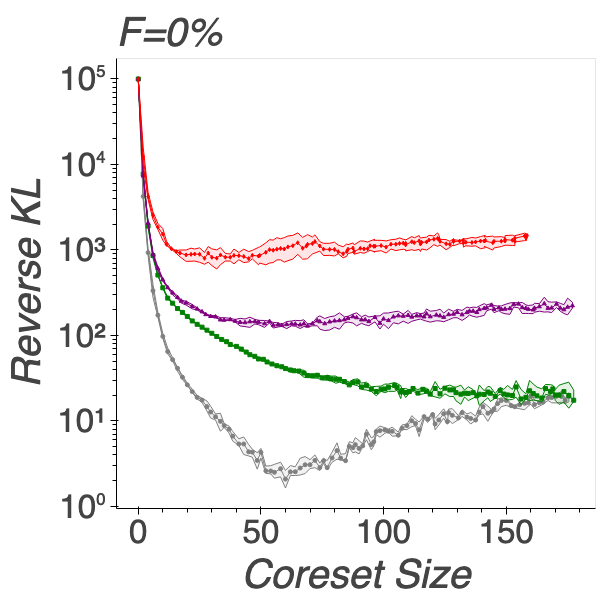
\includegraphics[width=.325\textwidth]{\MyPath/figs/comp_beta_F0_KLDvsCstSize.png}
		\centering
		\hfill
		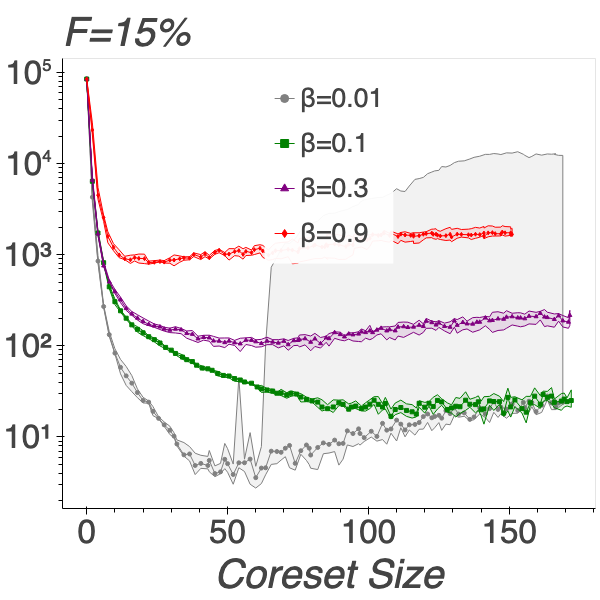
\includegraphics[width=.325\textwidth]{\MyPath/figs/comp_beta_F15_KLDvsCstSize.png}
		\centering
		\hfill
		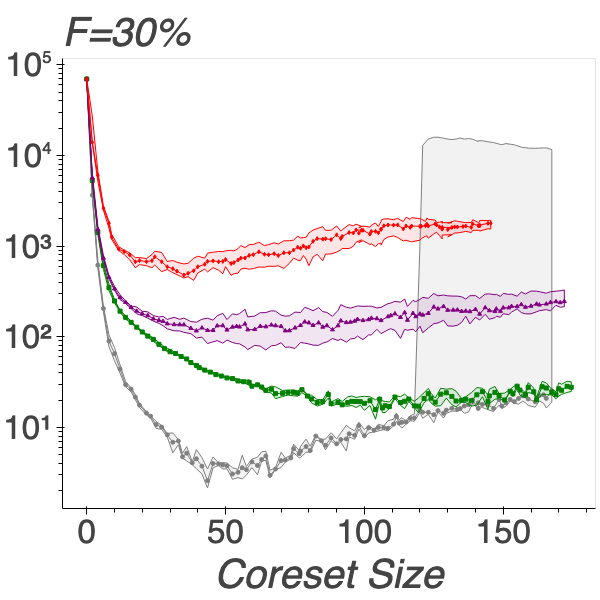
\includegraphics[width=.325\textwidth]{\MyPath/figs/comp_beta_F30_KLDvsCstSize.png}
		\centering
		\caption{(b)~Logistic regression}
		\centering 
		\hfill
		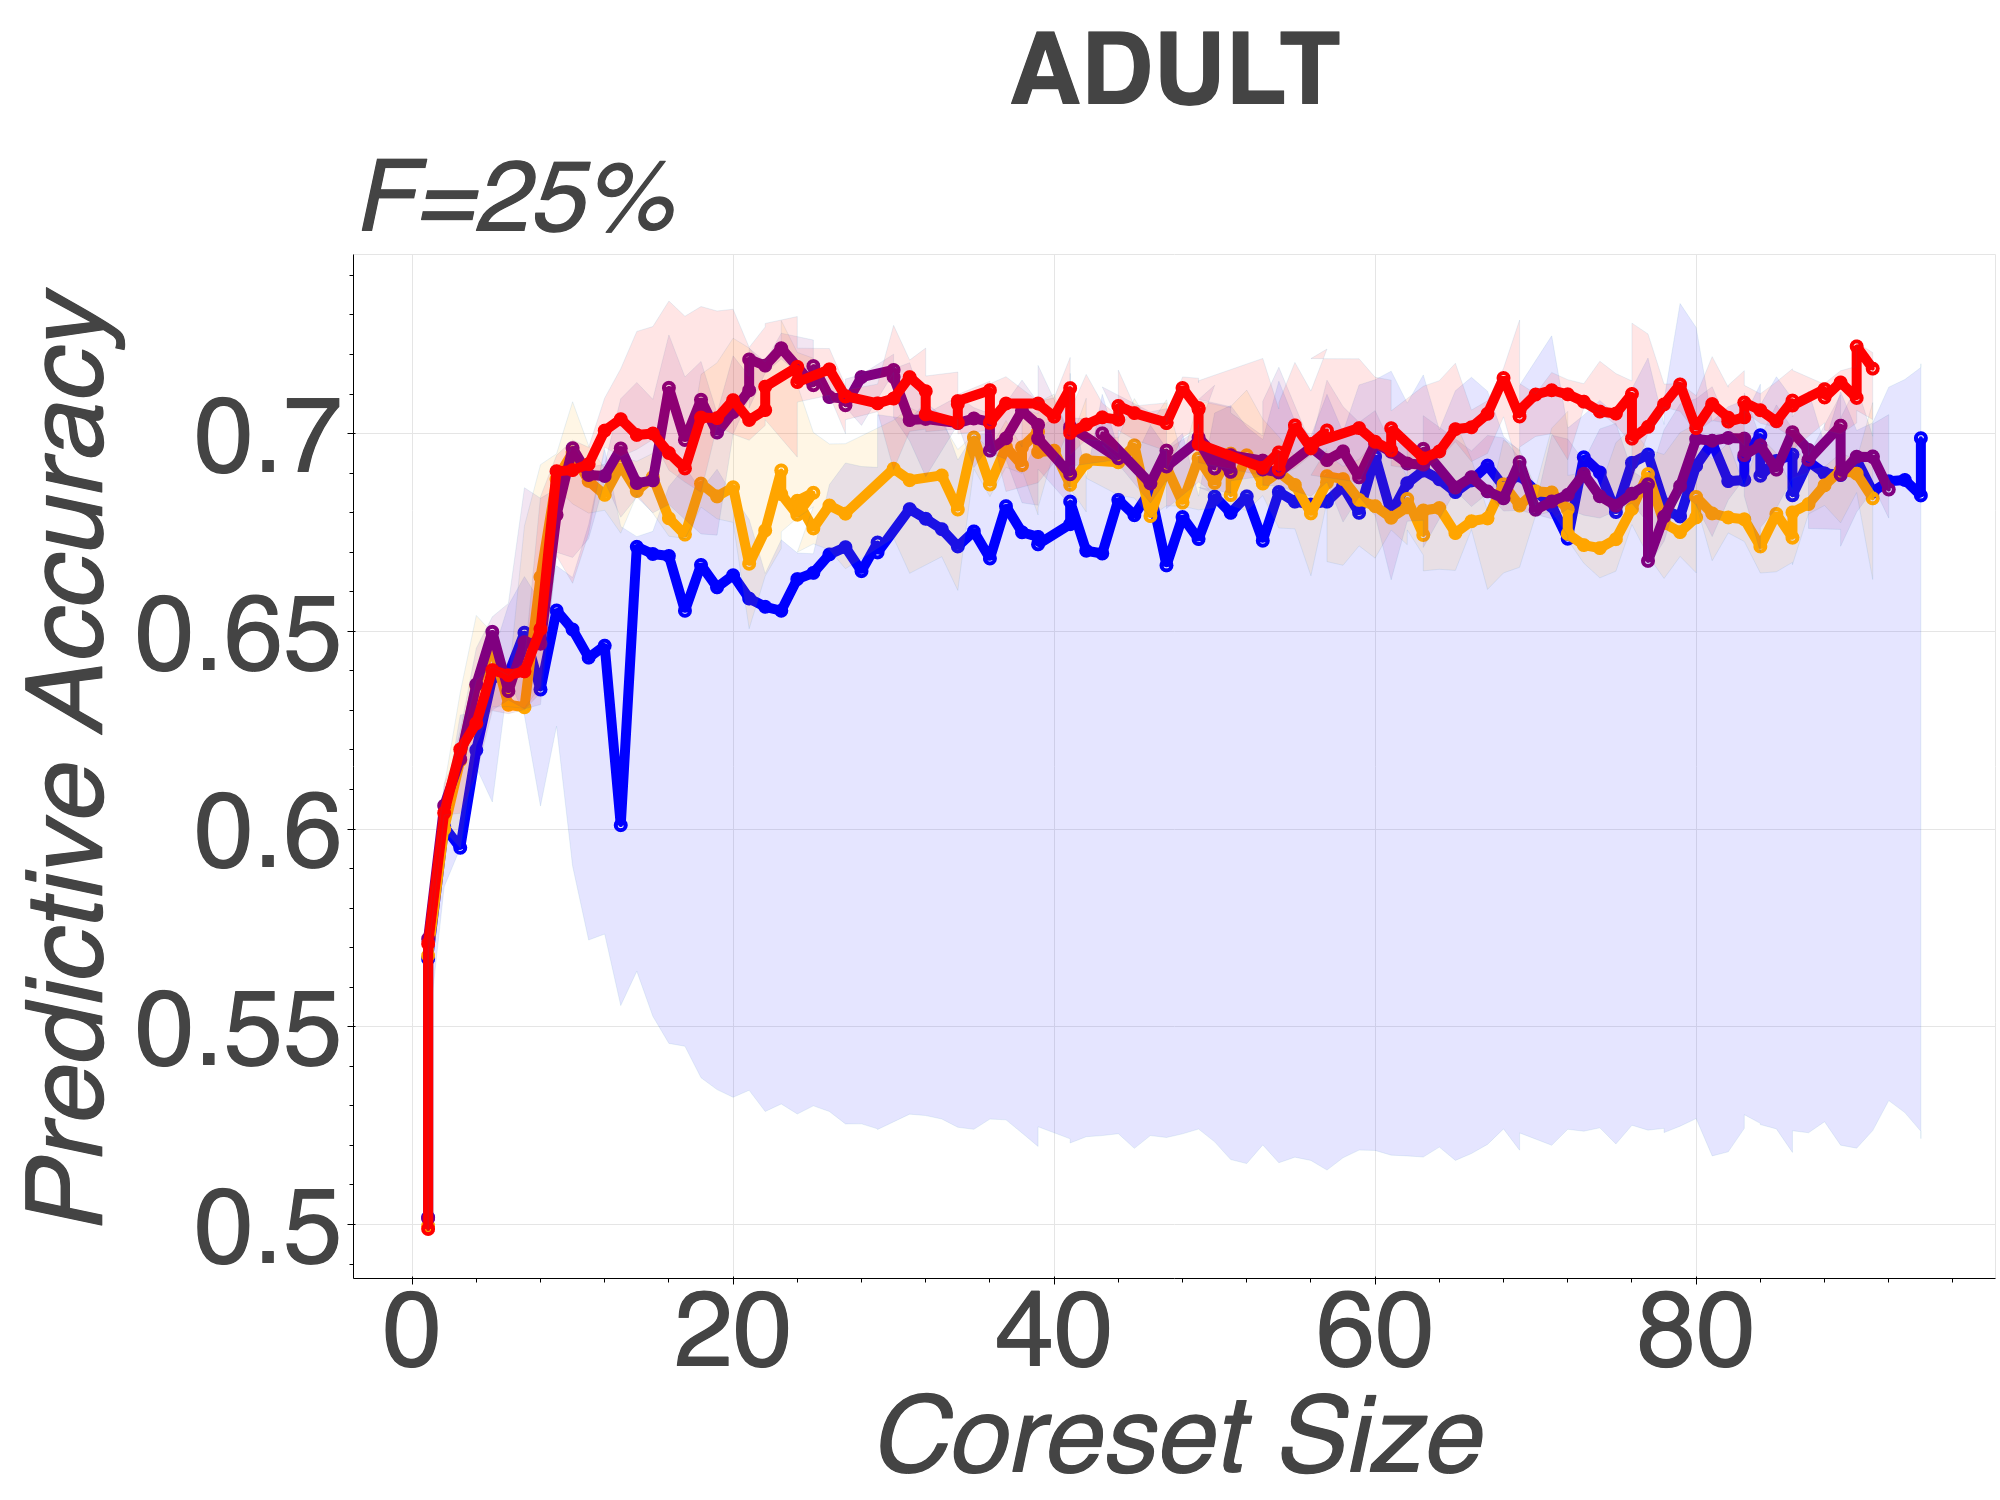
\includegraphics[width=.325\textwidth]{\MyPath/figs/comp_beta_F_25_adult_ACCvssz.png}
		\centering
		\hfil
		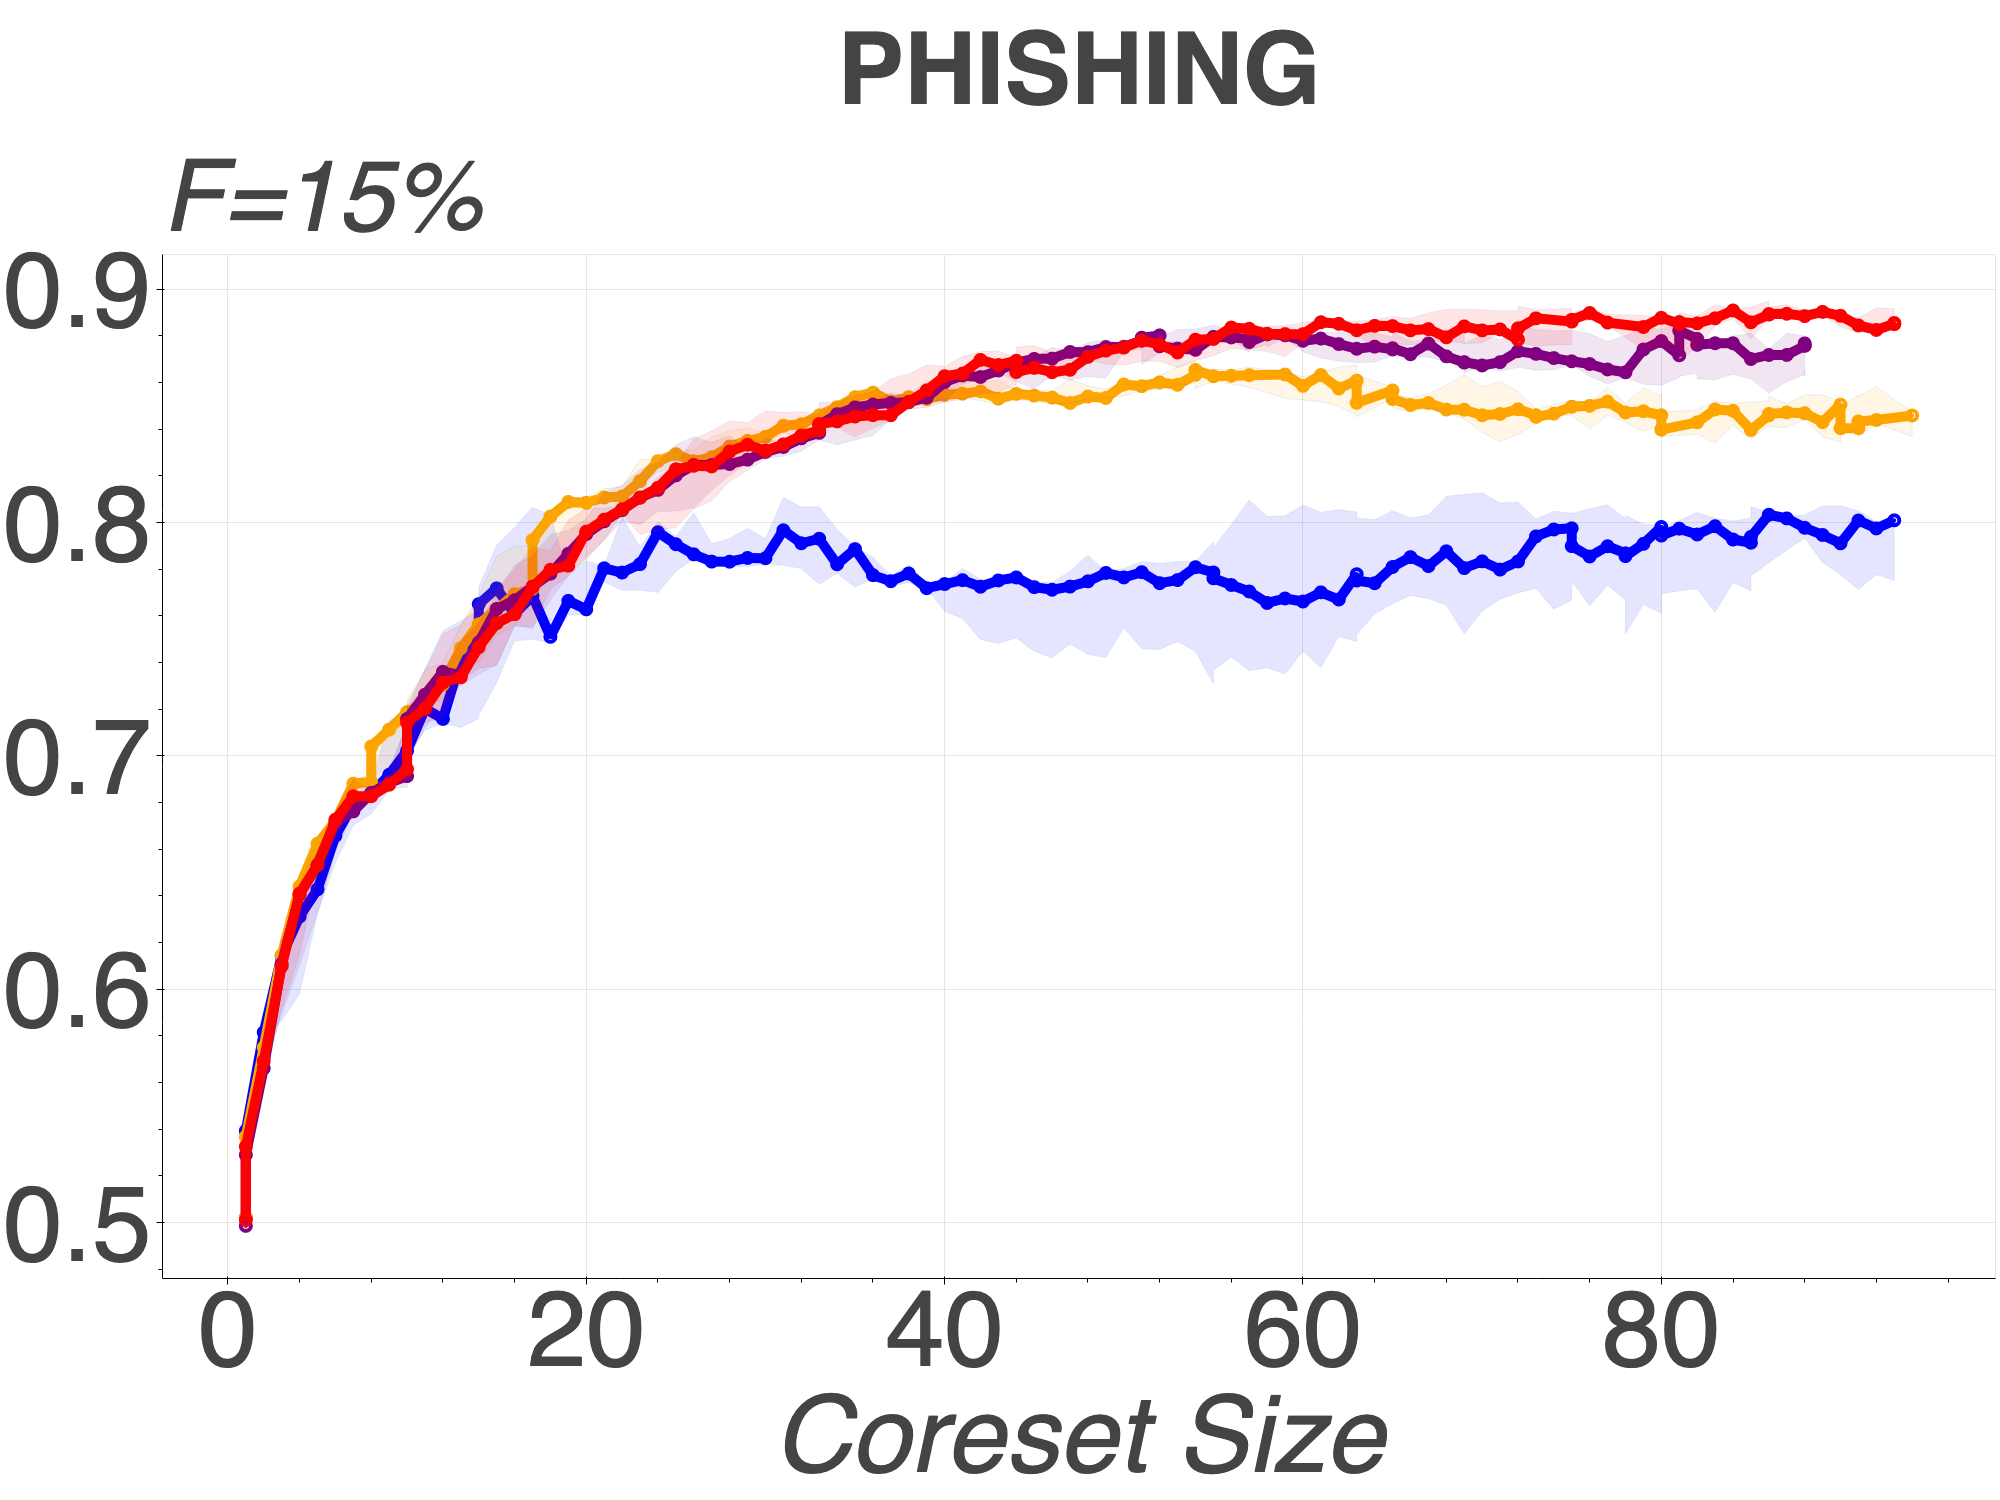
\includegraphics[width=.325\textwidth]{\MyPath/figs/comp_beta_F_15_phish_ACCvssz.png}
		\centering
		\hfill
		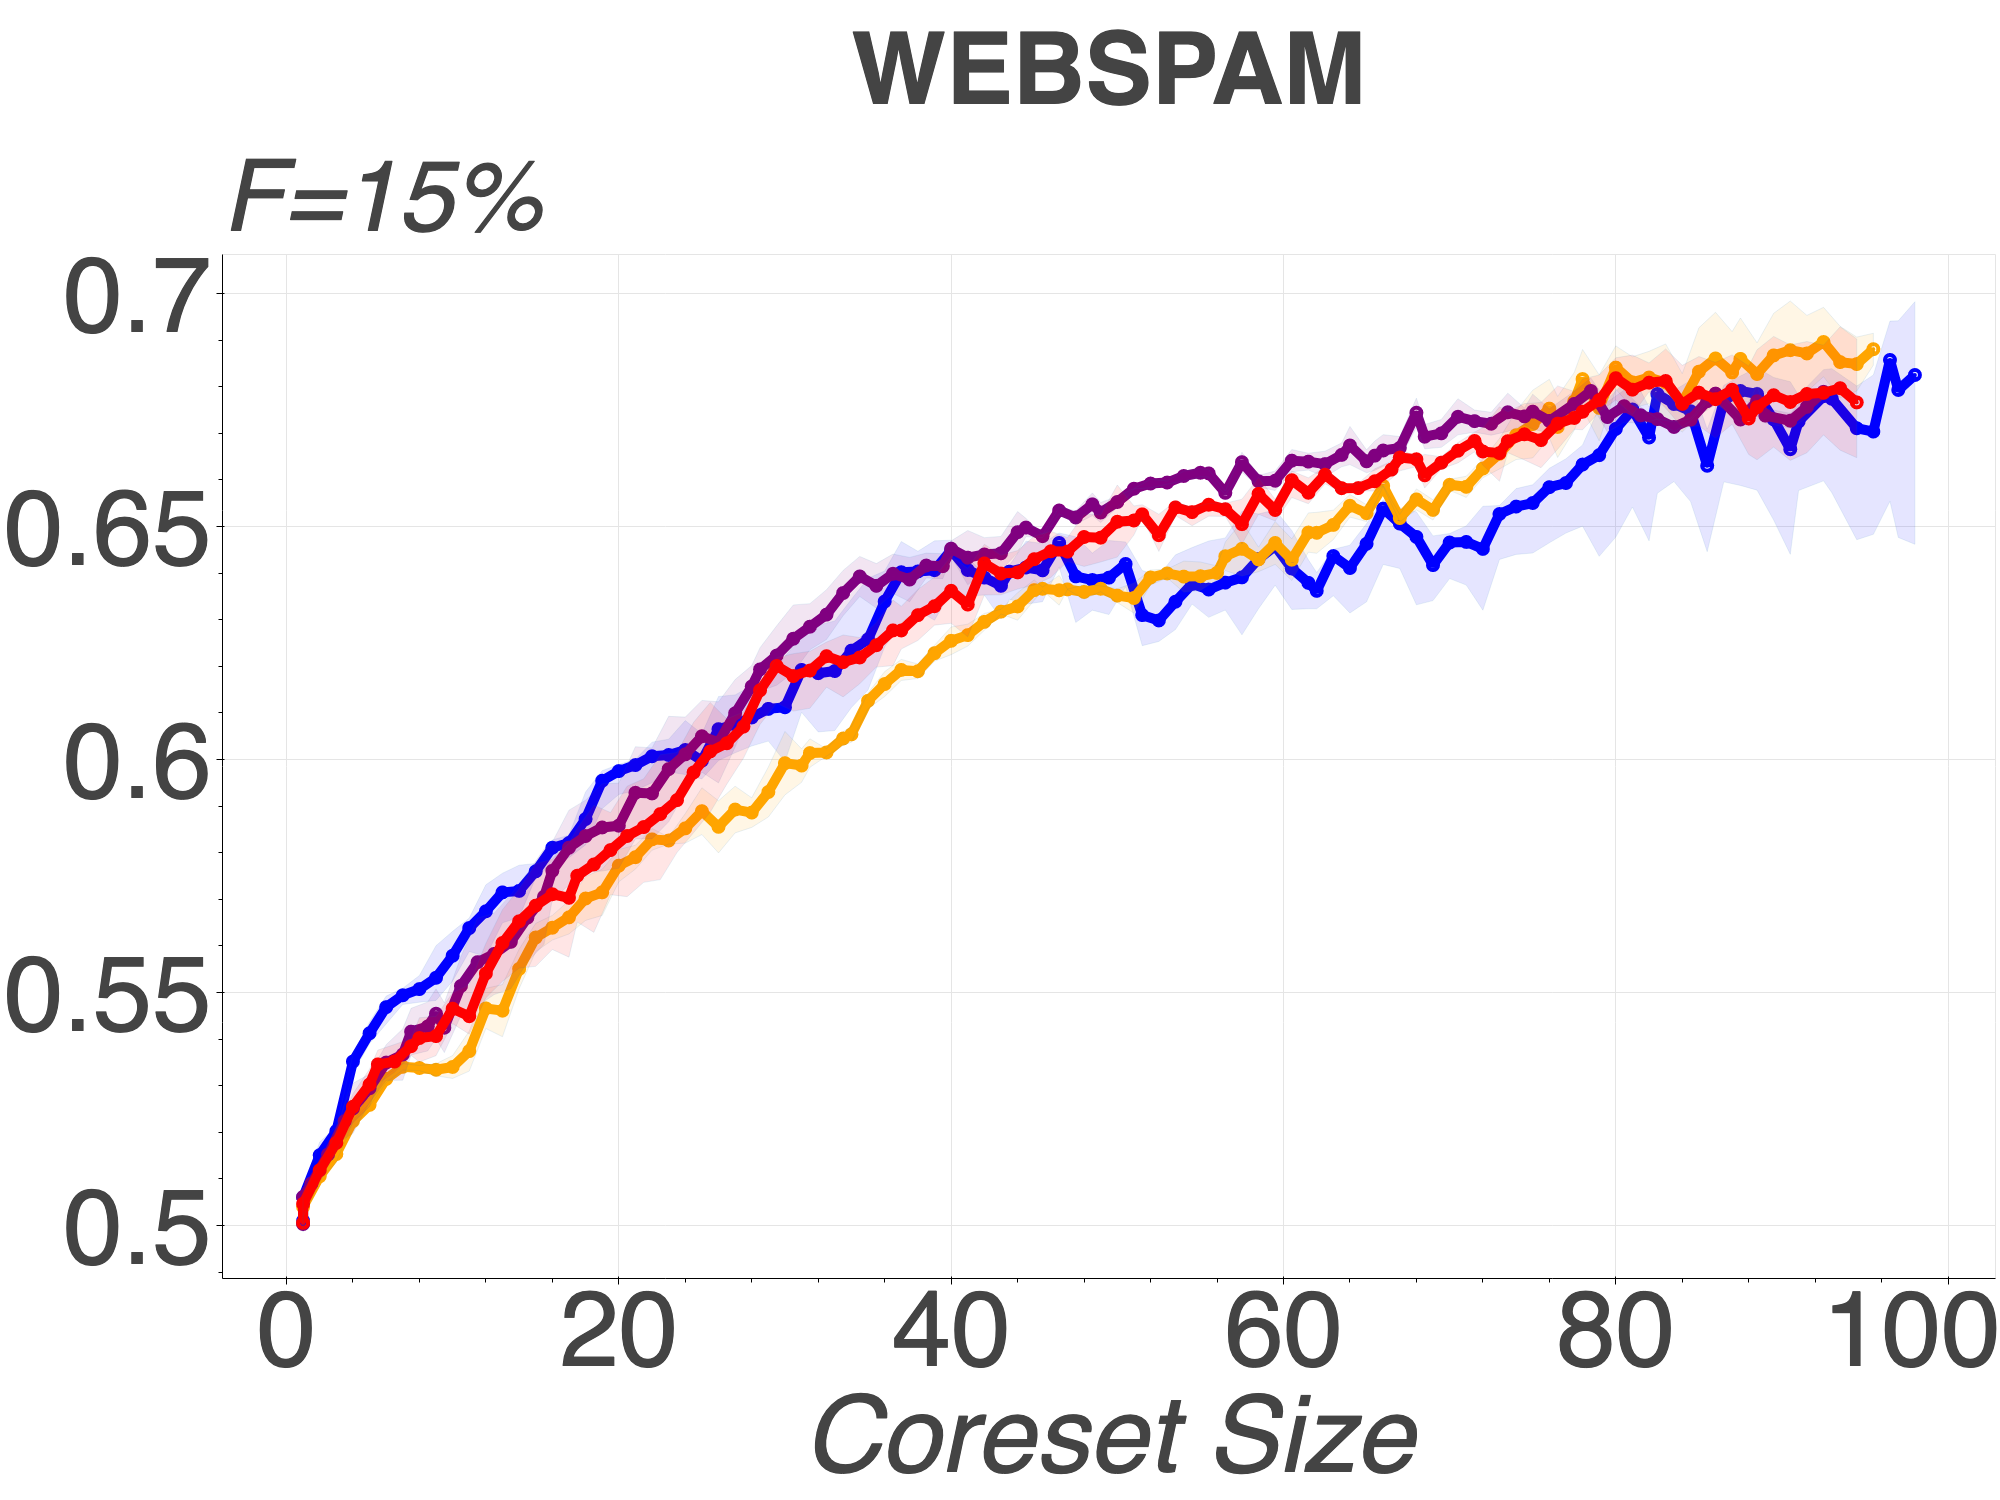
\includegraphics[width=.325\textwidth]{\MyPath/figs/comp_beta_F_15_webspam_ACCvssz.png}
		\centering
		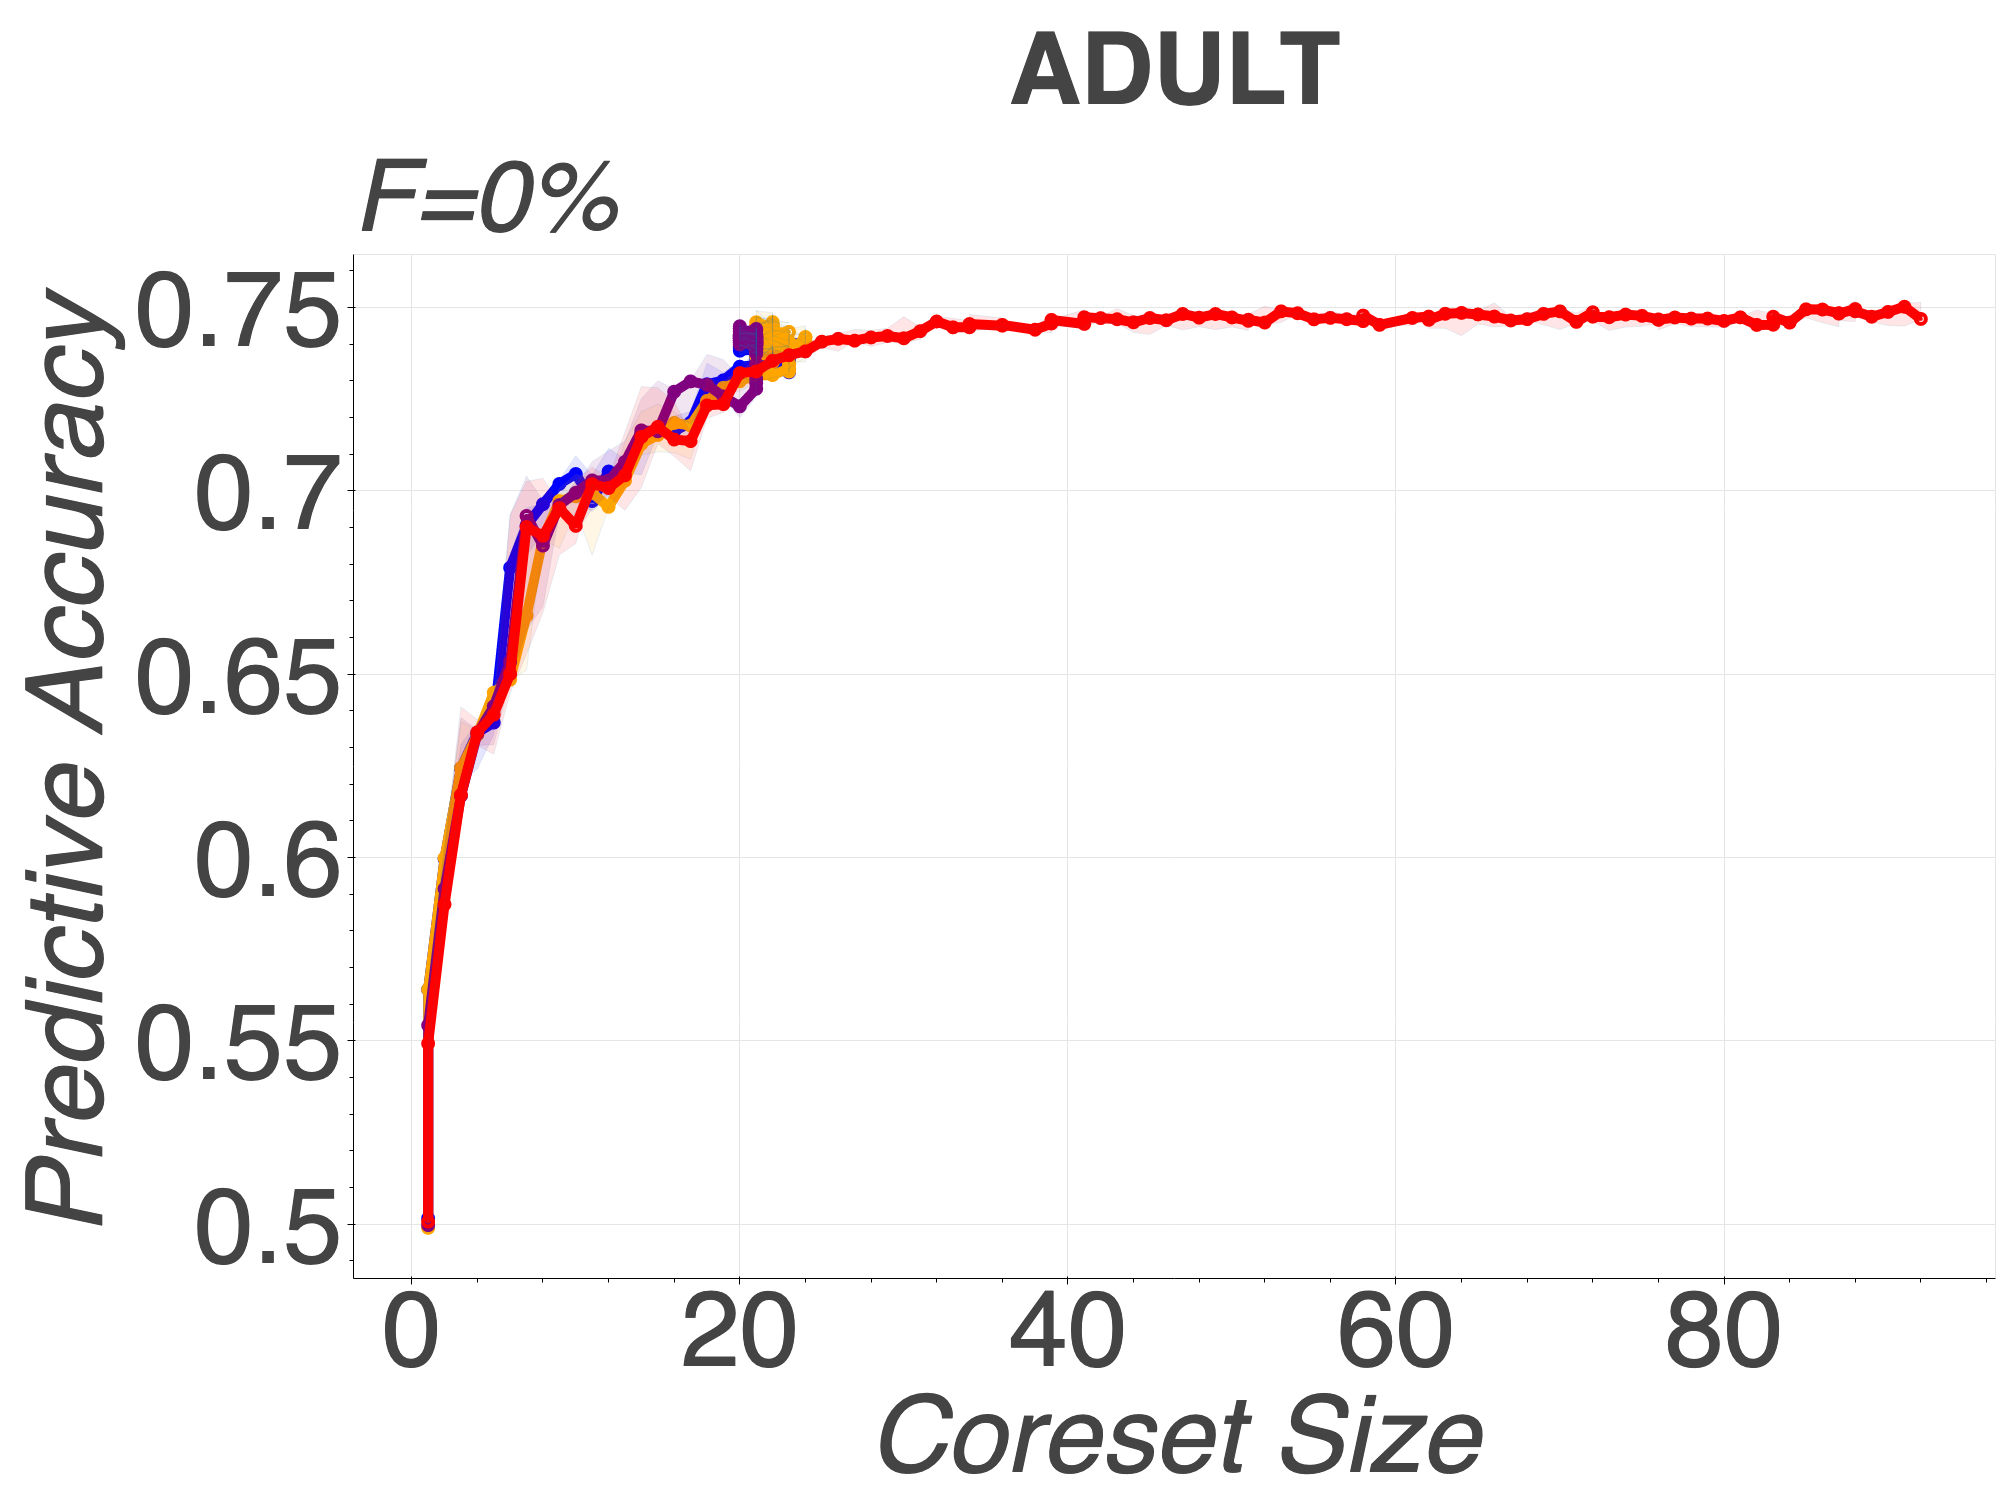
\includegraphics[width=.325\textwidth]{\MyPath/figs/comp_beta_F_0_adult_ACCvssz.png}
		\centering
		\hfill
		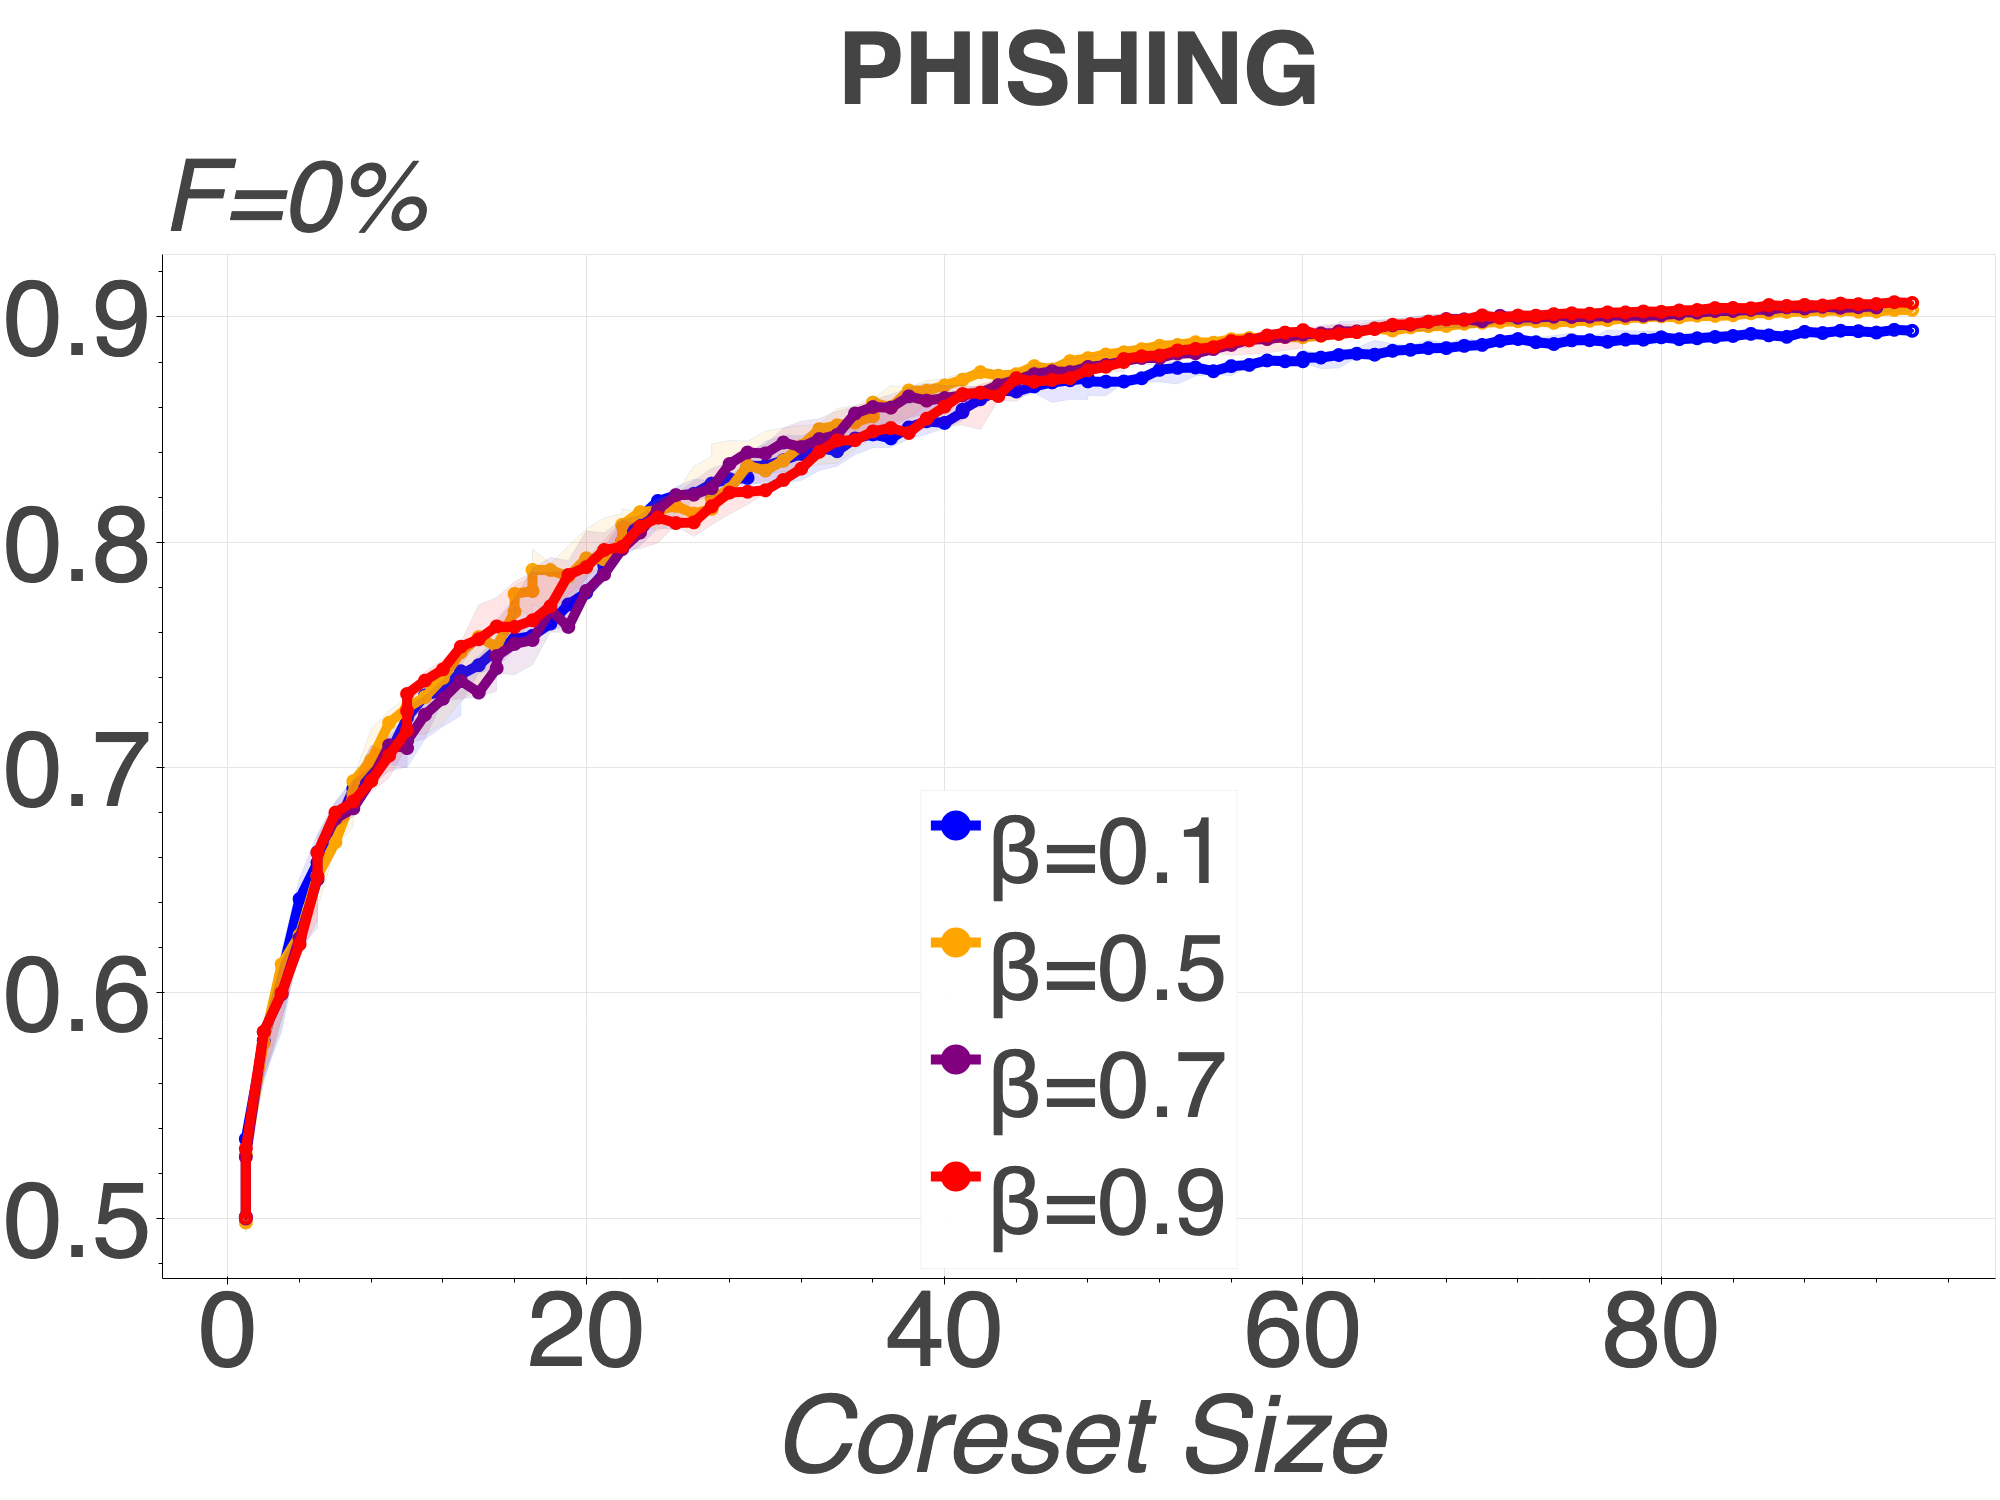
\includegraphics[width=.325\textwidth]{\MyPath/figs/comp_beta_F_0_phish_ACCvssz.png}
		\centering
		\hfill
		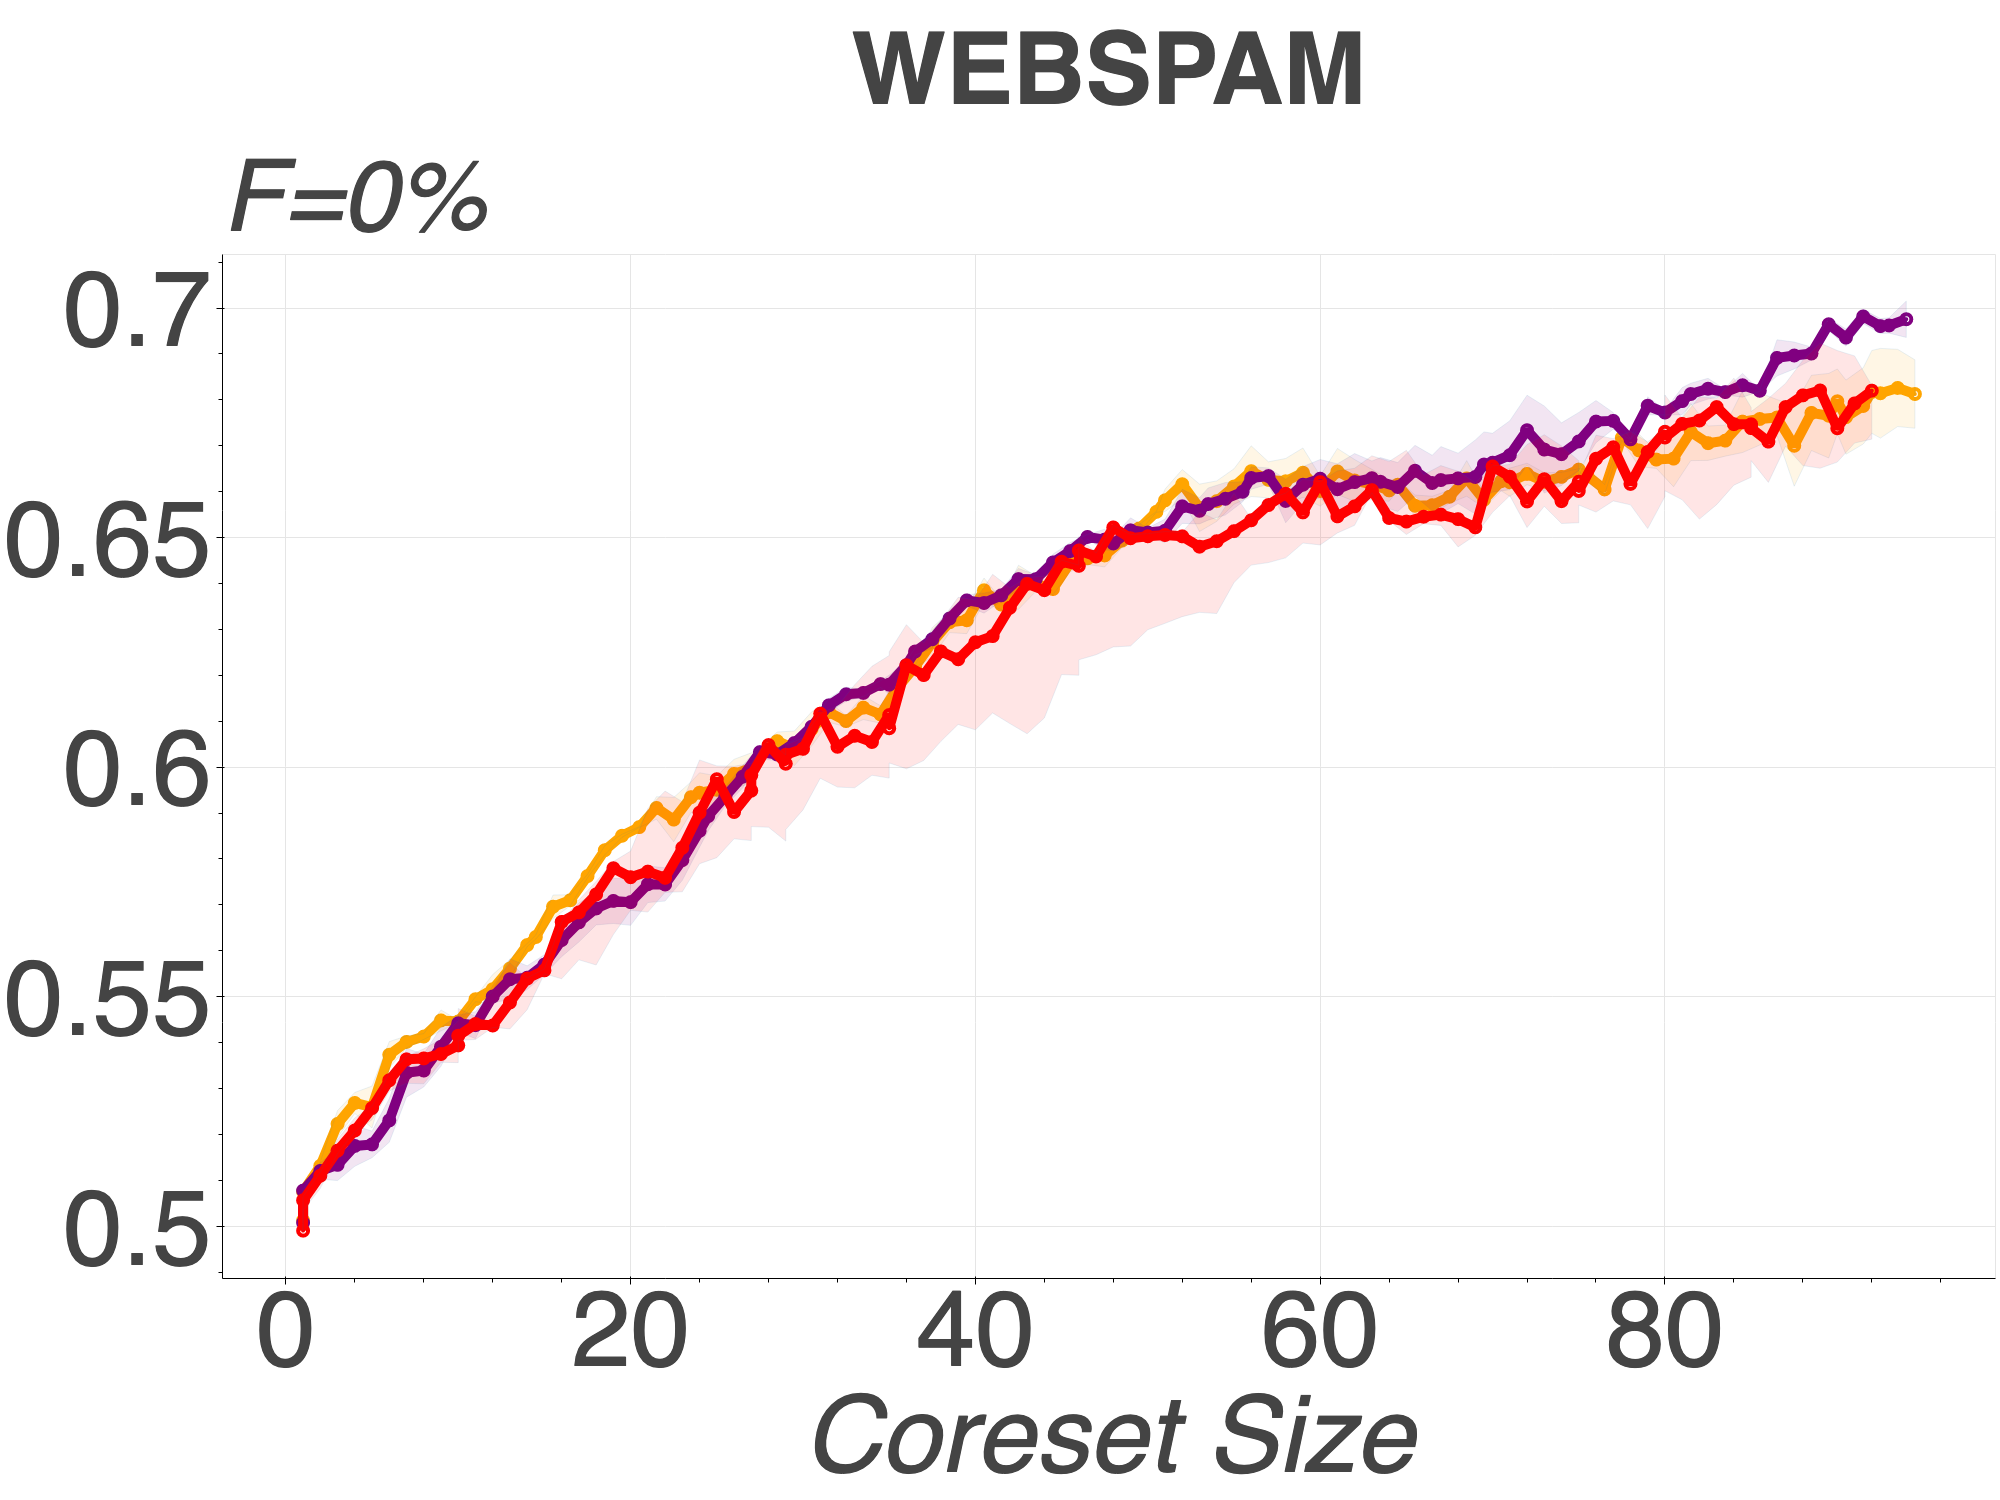
\includegraphics[width=.325\textwidth]{\MyPath/figs/comp_beta_F_0_webspam_ACCvssz.png}
		\centering
		\caption{(c)~Neural linear regression}
		\centering
		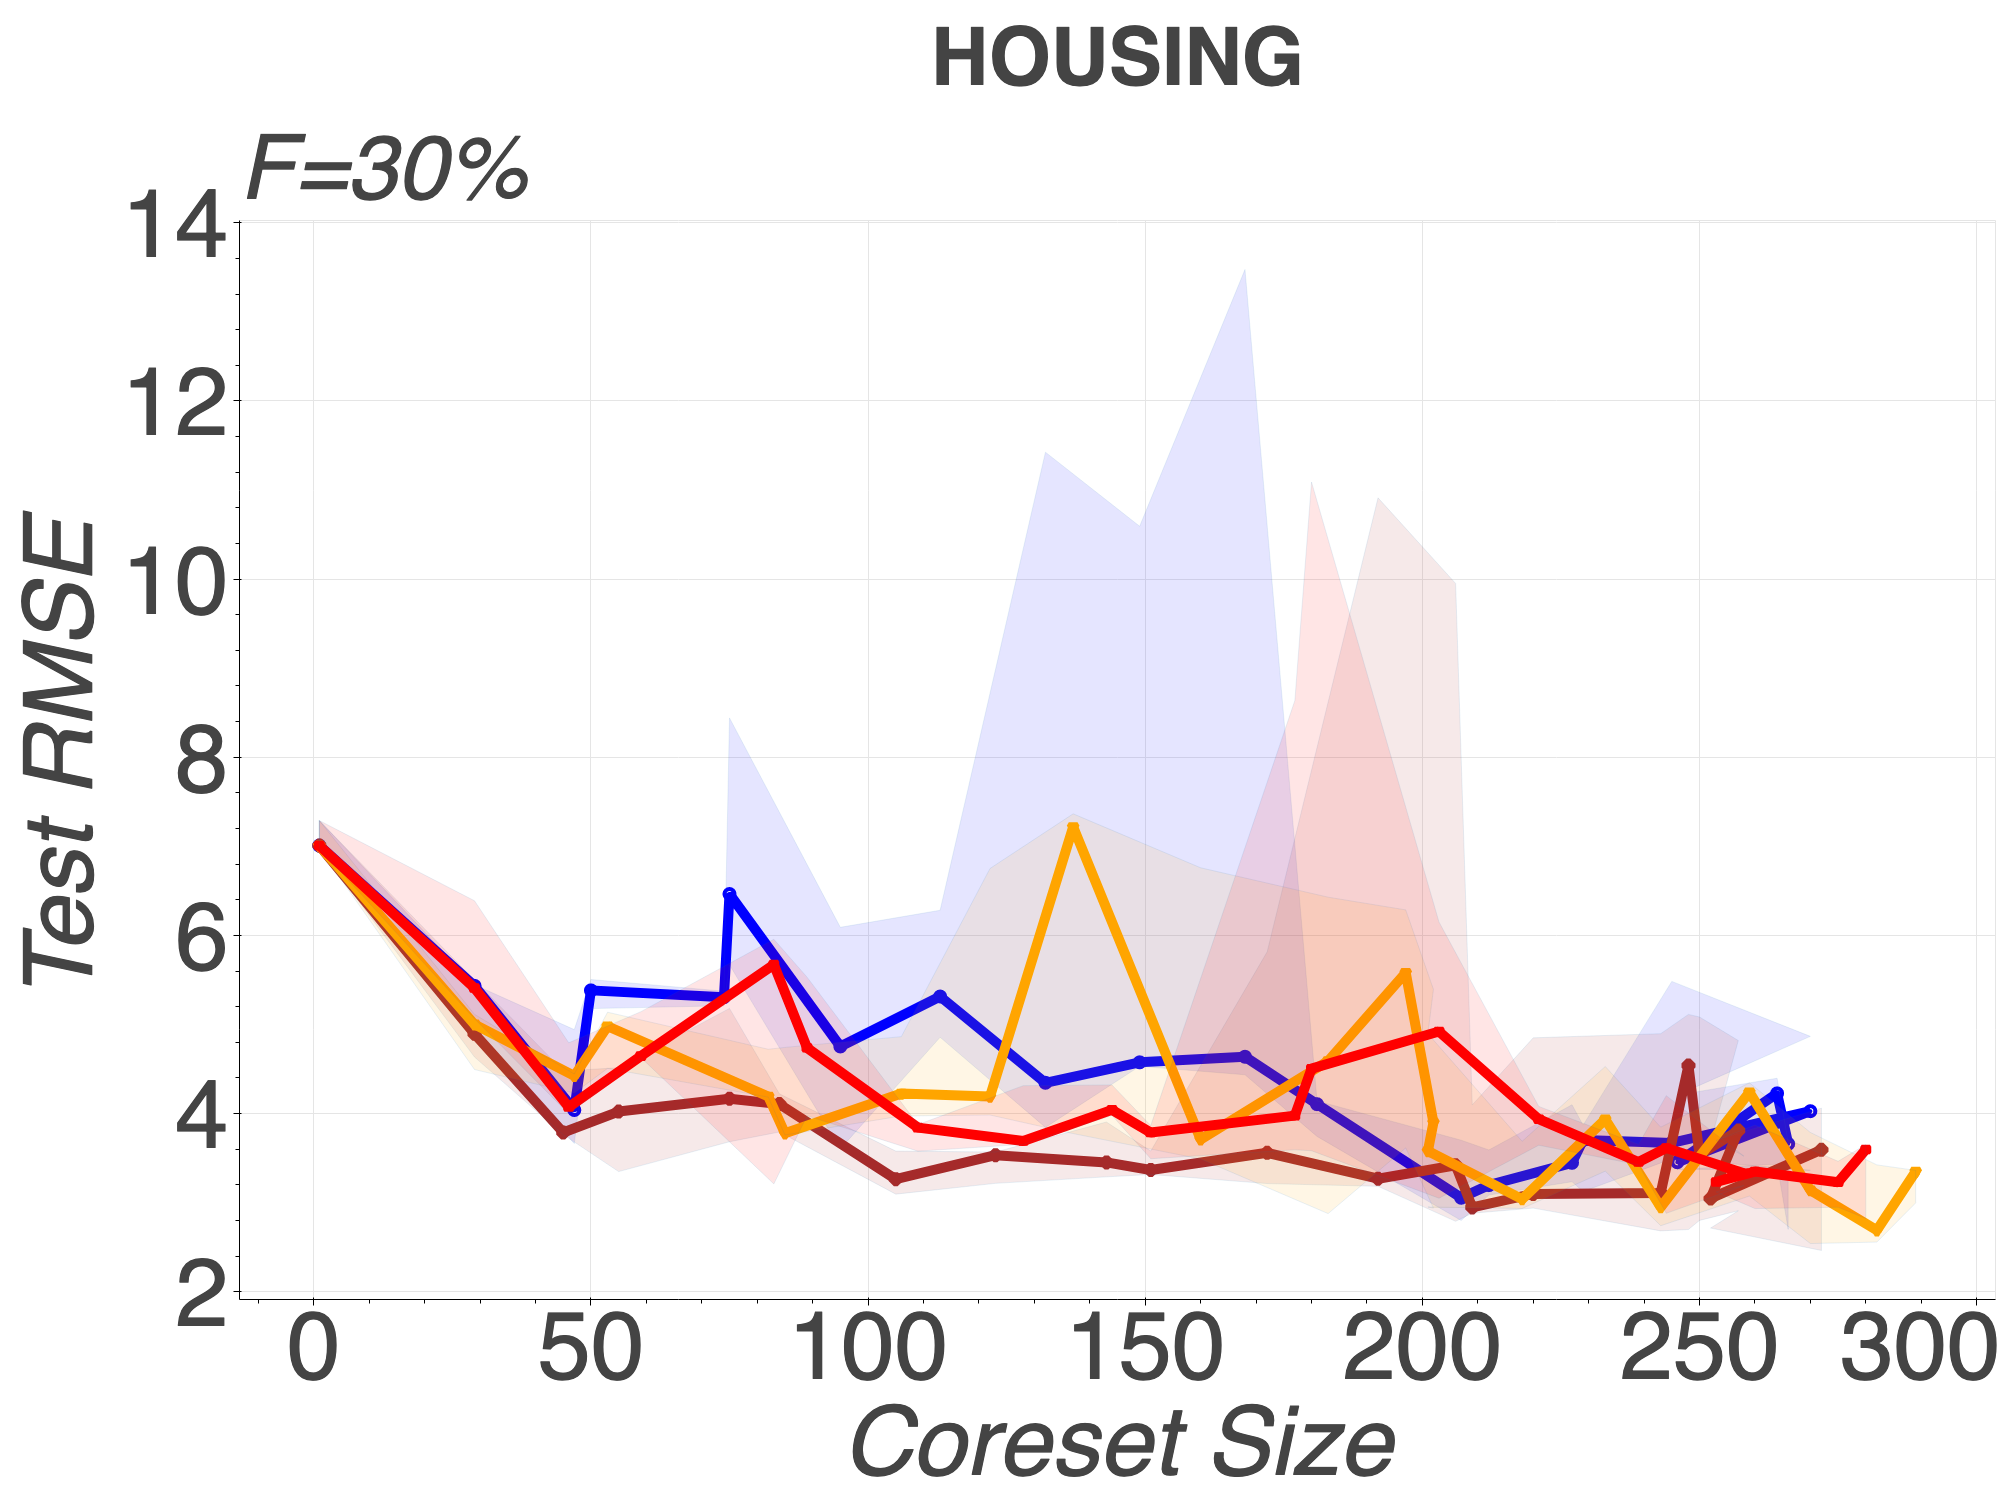
\includegraphics[width=.33\textwidth]{\MyPath/figs/comp_beta_F_boston09_01_30_RMSEvssz.png}
		\centering
		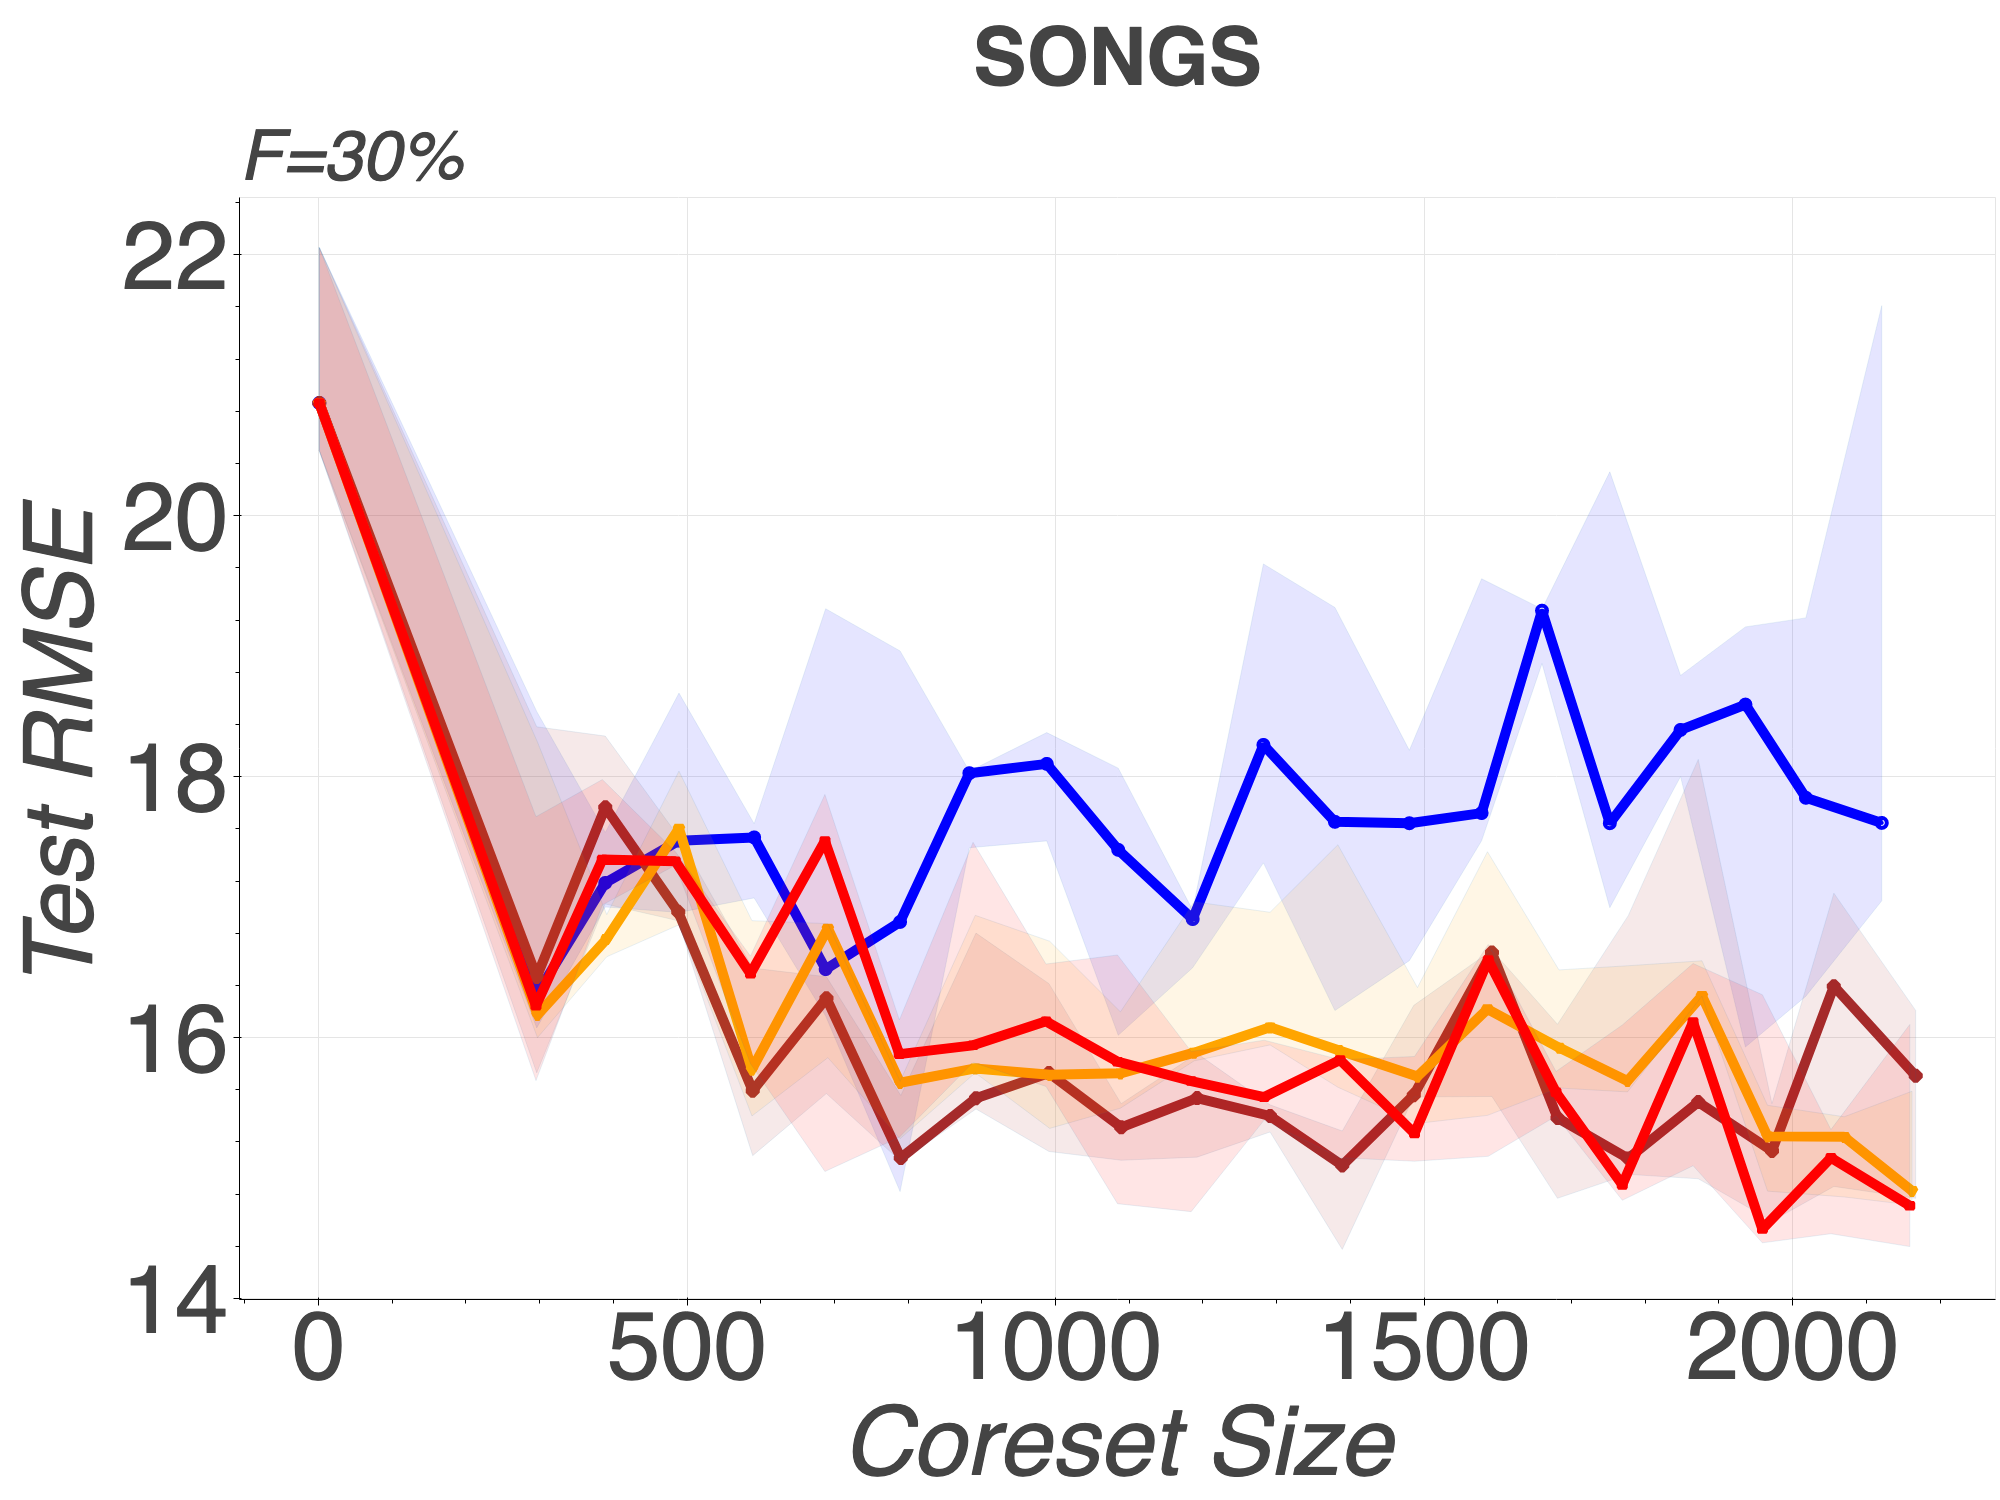
\includegraphics[width=.33\textwidth]{\MyPath/figs/comp_beta_F_year09_01_30_RMSEvssz.png}
		\centering
		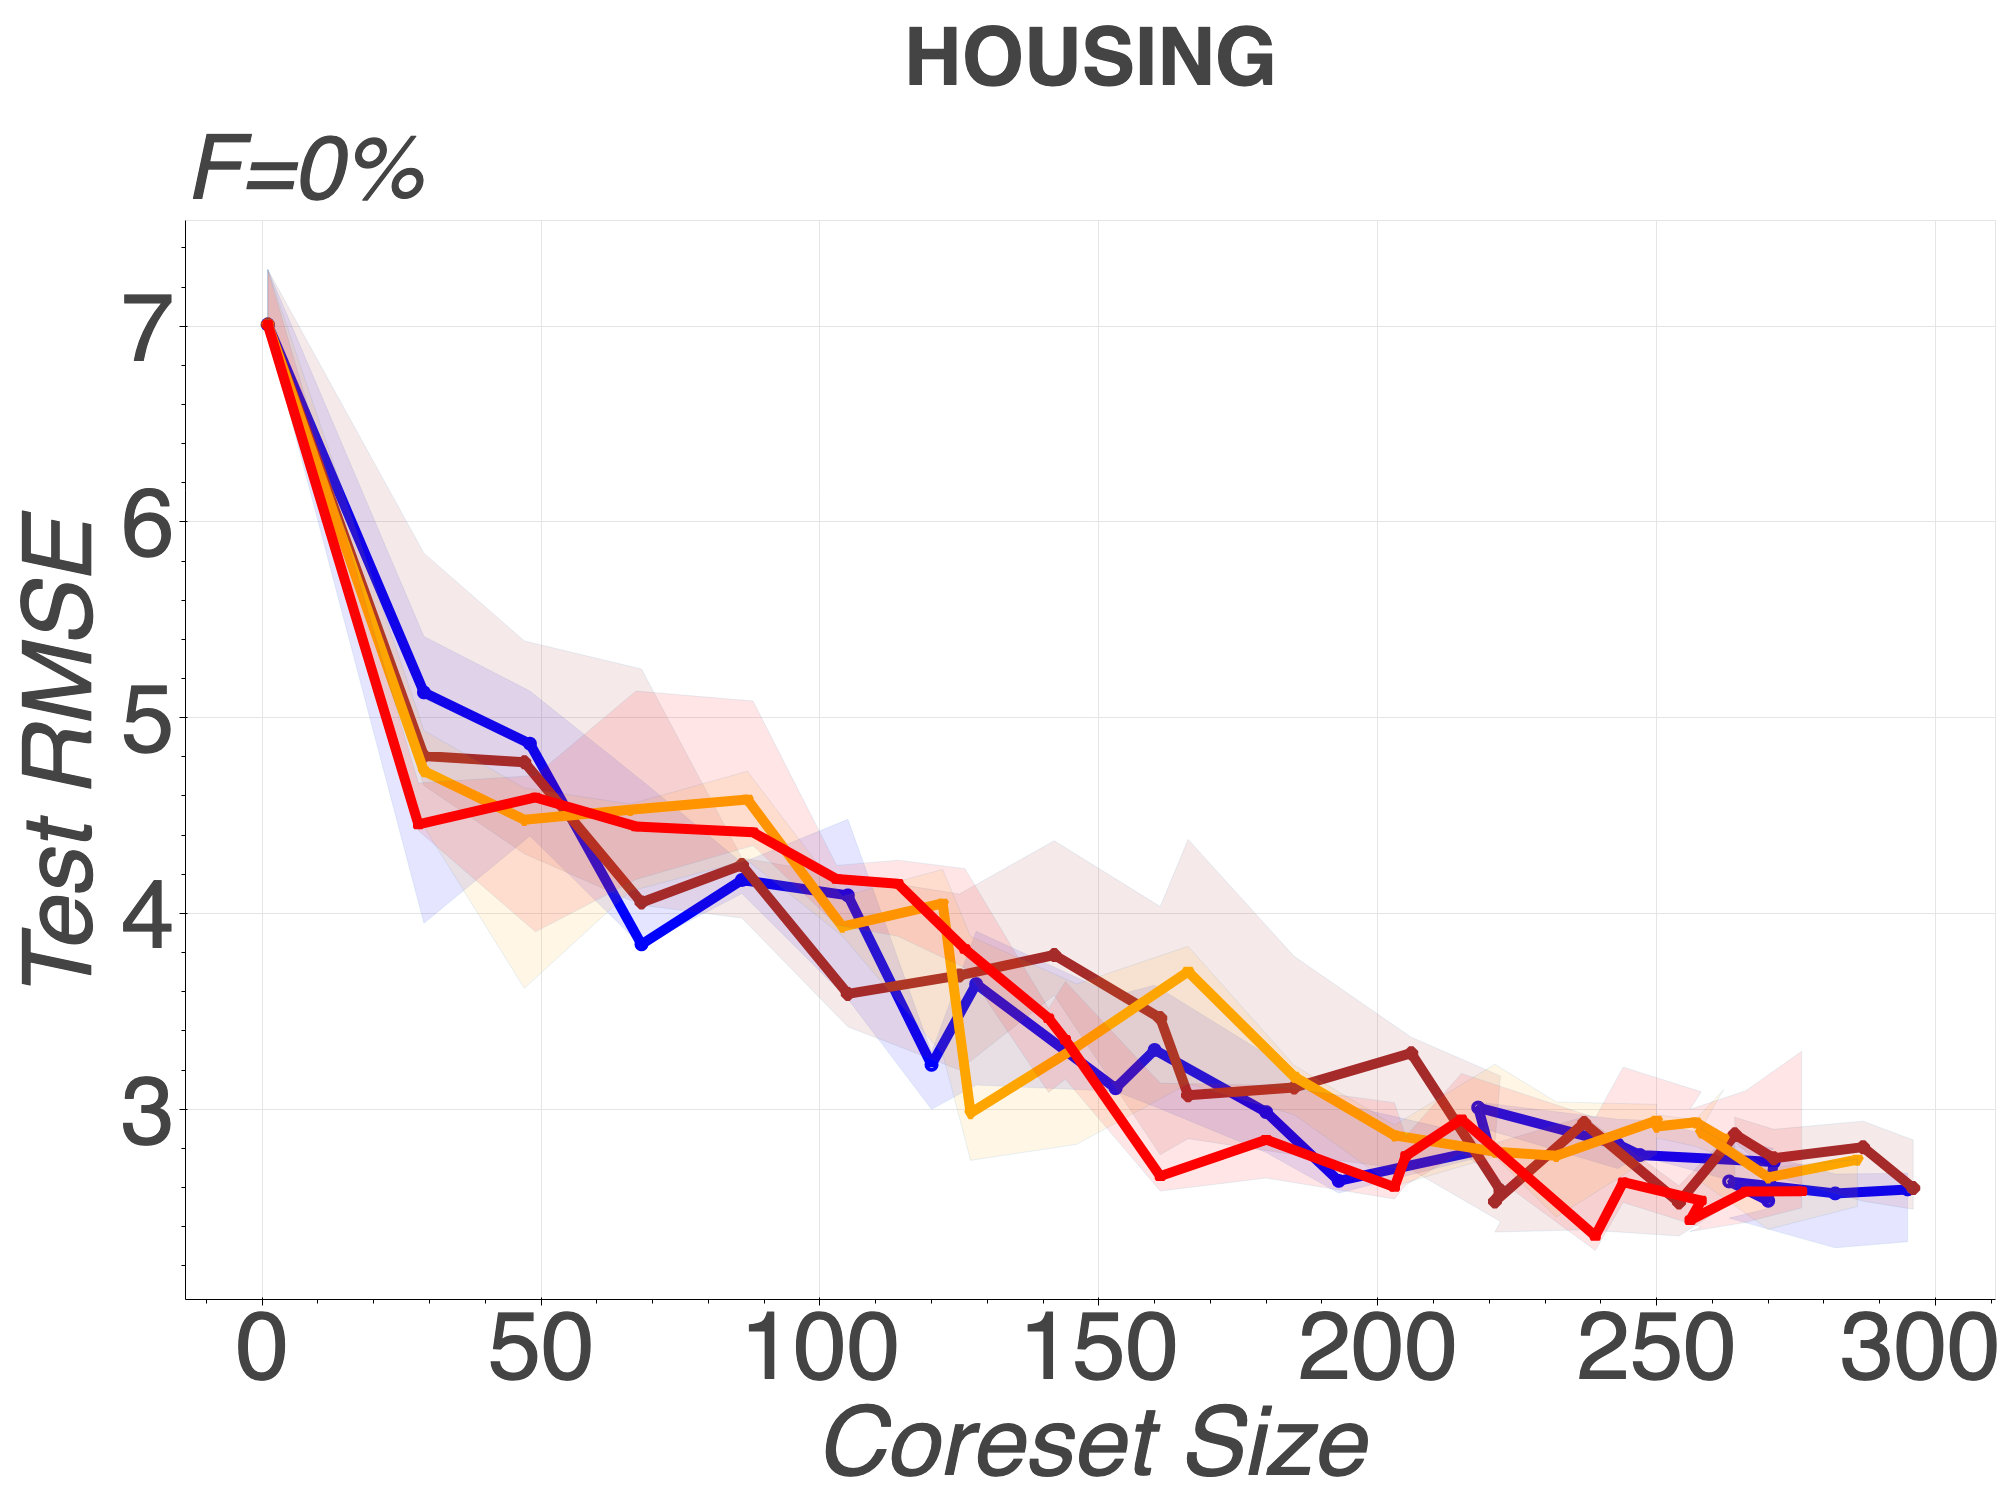
\includegraphics[width=.33\textwidth]{\MyPath/figs/comp_beta_F_boston09_01_0_RMSEvssz.png}
		\centering
		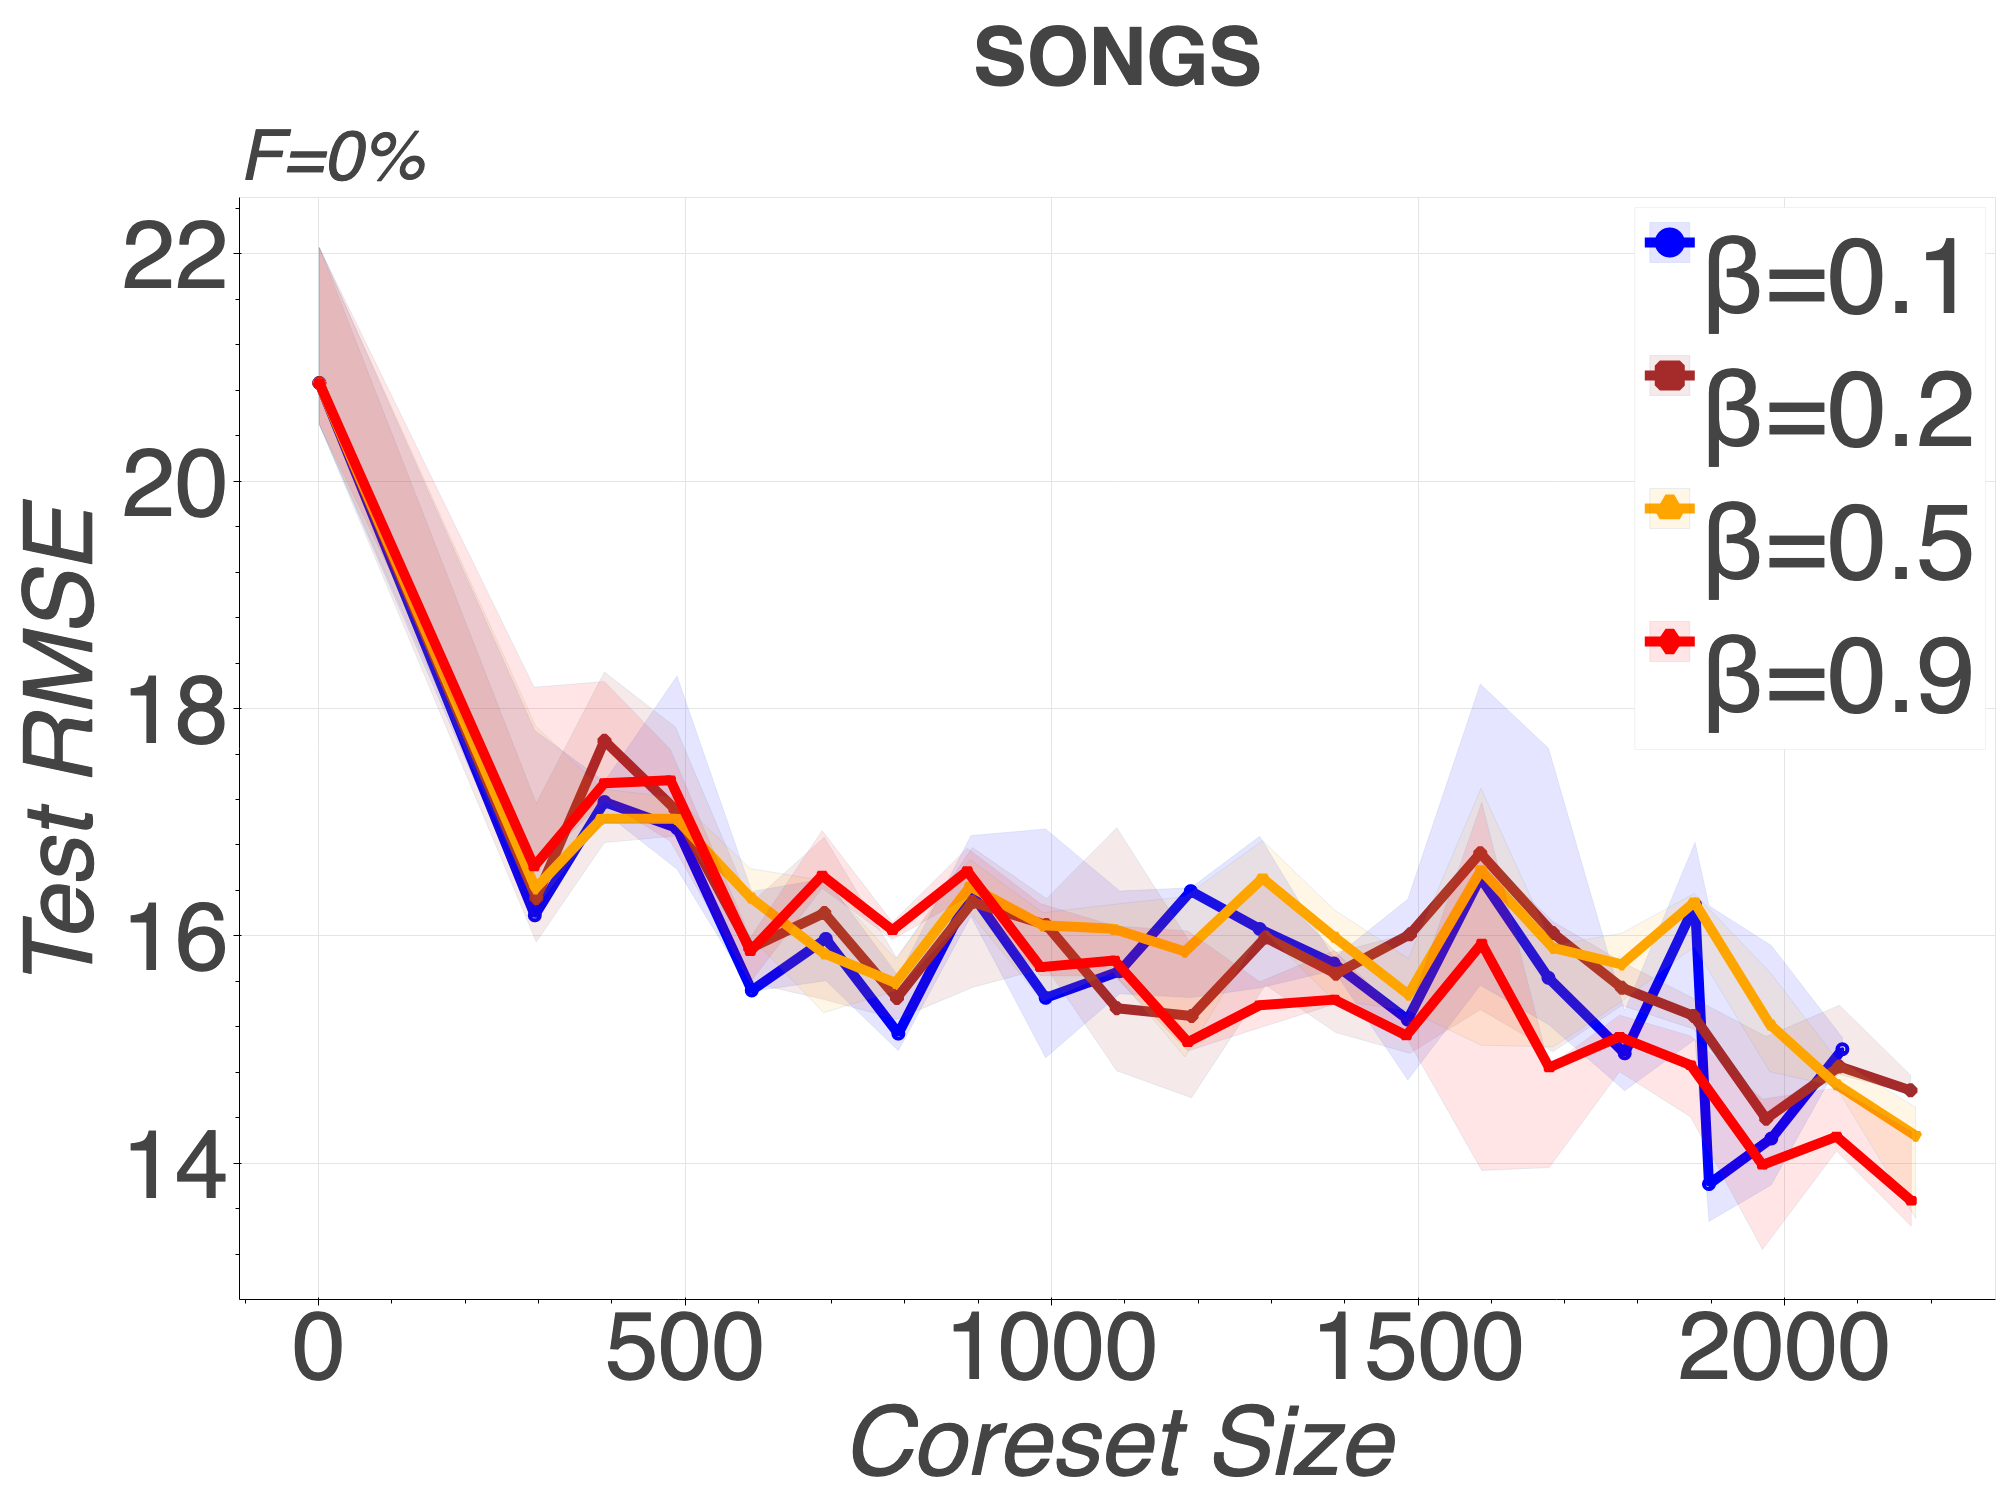
\includegraphics[width=.33\textwidth]{\MyPath/figs/comp_beta_F_year09_01_0_RMSEvssz.png}
	\end{subfigure}	
	\centering
	\caption{Reverse KL divergence between \bcores{} and true posterior (the latter computed on clean data) for varying values of the robustness hyperparameter $\beta$. Results are averaged over $5$ trials. Solid lines display the median KL divergence, with shaded areas showing $25\textsuperscript{th}$ and $75\textsuperscript{th}$ percentiles of KL divergence.}
	\label{fig:beta_sens}
\end{figure}
